\subsection{Descripci\'on del Escenario}
	\par Al igual que el escenario anterior, esta es una red laboral, pero con características muy diferentes. La red pertenece a una oficina de desarrollo de software y hardware con 14 personas. También hay un servidor de archivos, uno con maquinas virtuales y uno con bases de datos, 1 bridge wireless (independiente del router) y varios dispositivos de hardware conectados a la misma. La red es 10.10.0.0/24, teniendo el gateway la IP 10.10.0.1. 
     \par Se capturaron paquetes arp durante 5 horas, mediante una interfaz de red Ethernet.
     
\subsection{An\'alisis de datos obtenidos}
	\par Comenzamos realizando un grafo dirigido, en el cual los nodos son las direcciones IP, y los ejes representan pedidos arp ("who-has") de una IP fuente a una IP destino.
	\begin{figure}[!ht]
		\centering
		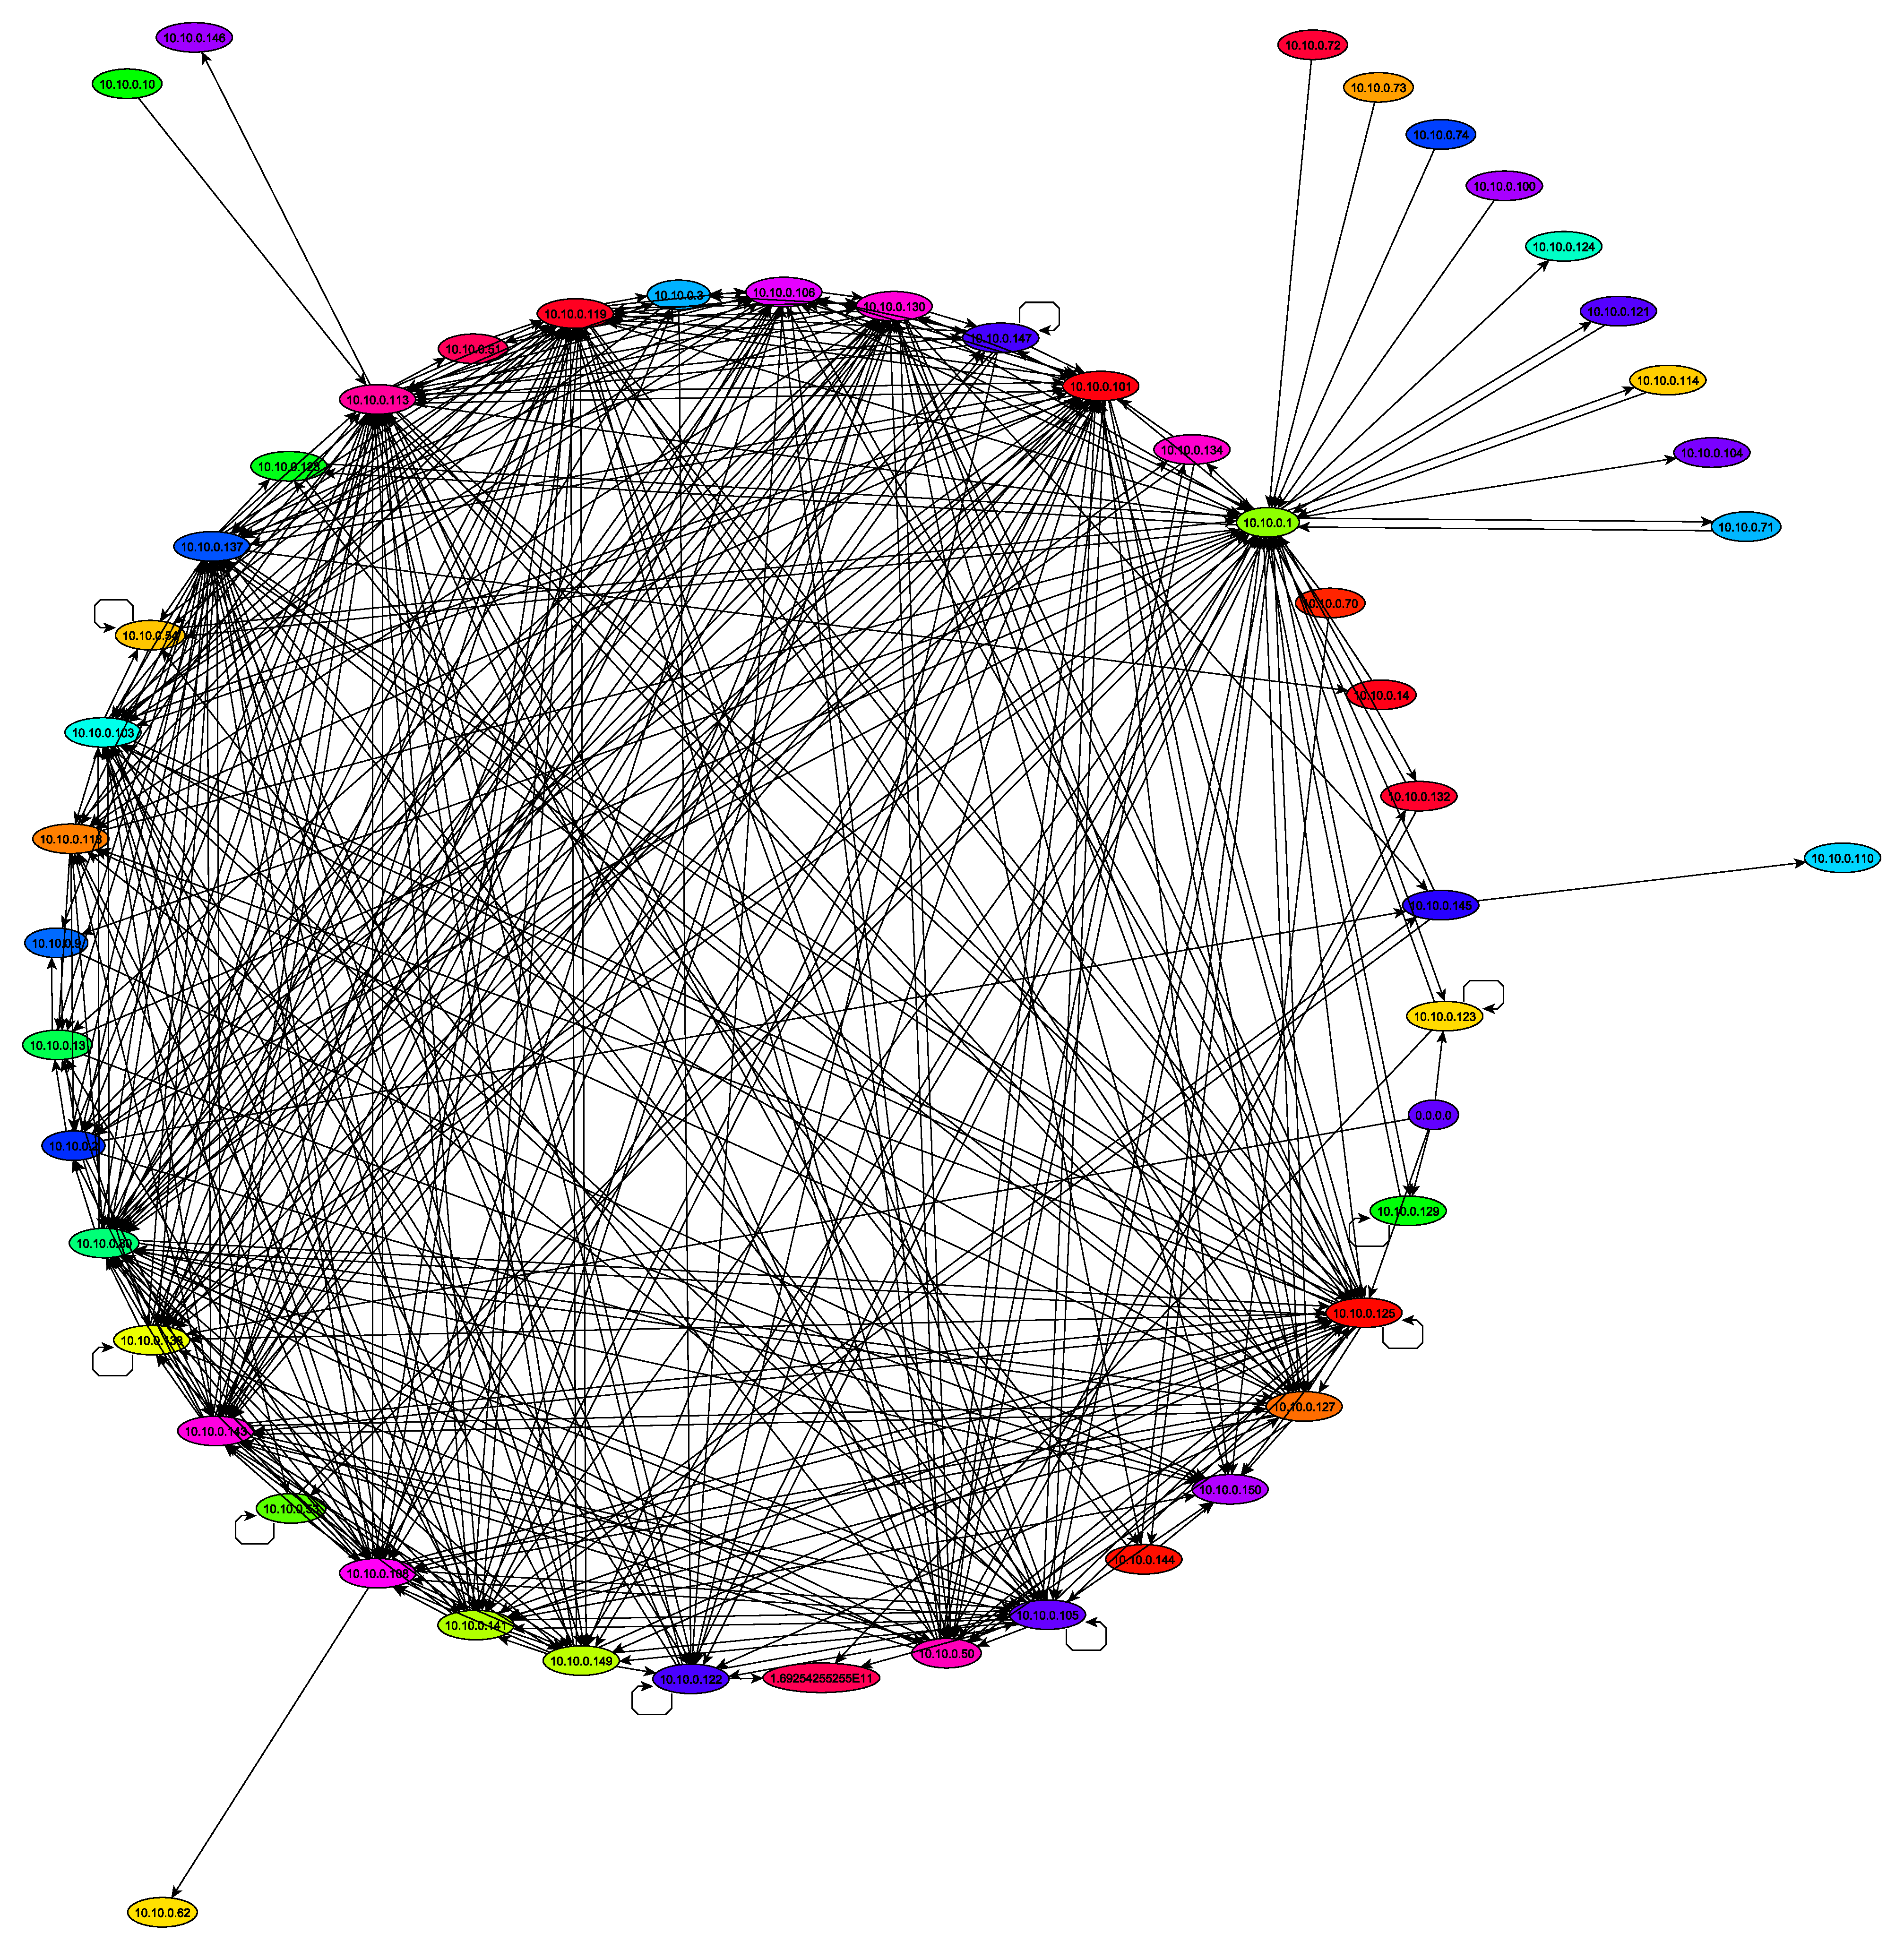
\includegraphics[width=0.5\textwidth]{img/graph/escenario_2/grafico_de_la_red.eps}
		\caption{Grafo de la red del Escenario 2}
		\label{fig:grafo_escenario2}
	\end{figure}
    
    A simple vista, este grafo no nos aporta demasiada información, pero el hecho de que sea una única gran componente conexa se corresponde con la configuración de la red. Inspeccionando las etiquetas de los nodos, observamos que efectivamente, todas las direcciones se encuentran en el rango 10.10.0.1-10.10.0.254, con excepción de dos casos particulares: la IP 0.0.0.0 y la IP 169.254.255.255. Más adelante nos concentraremos en estas dos direcciones. 
    \par Lo primero que nos interesó ver fue cuales fueron las IPs más pedidas, y cuales fueron las que más pedidos realizaron. Para esto, realizamos histogramas que reflejan visualmente esto:
\begin{figure}[!h]]
		\centering
		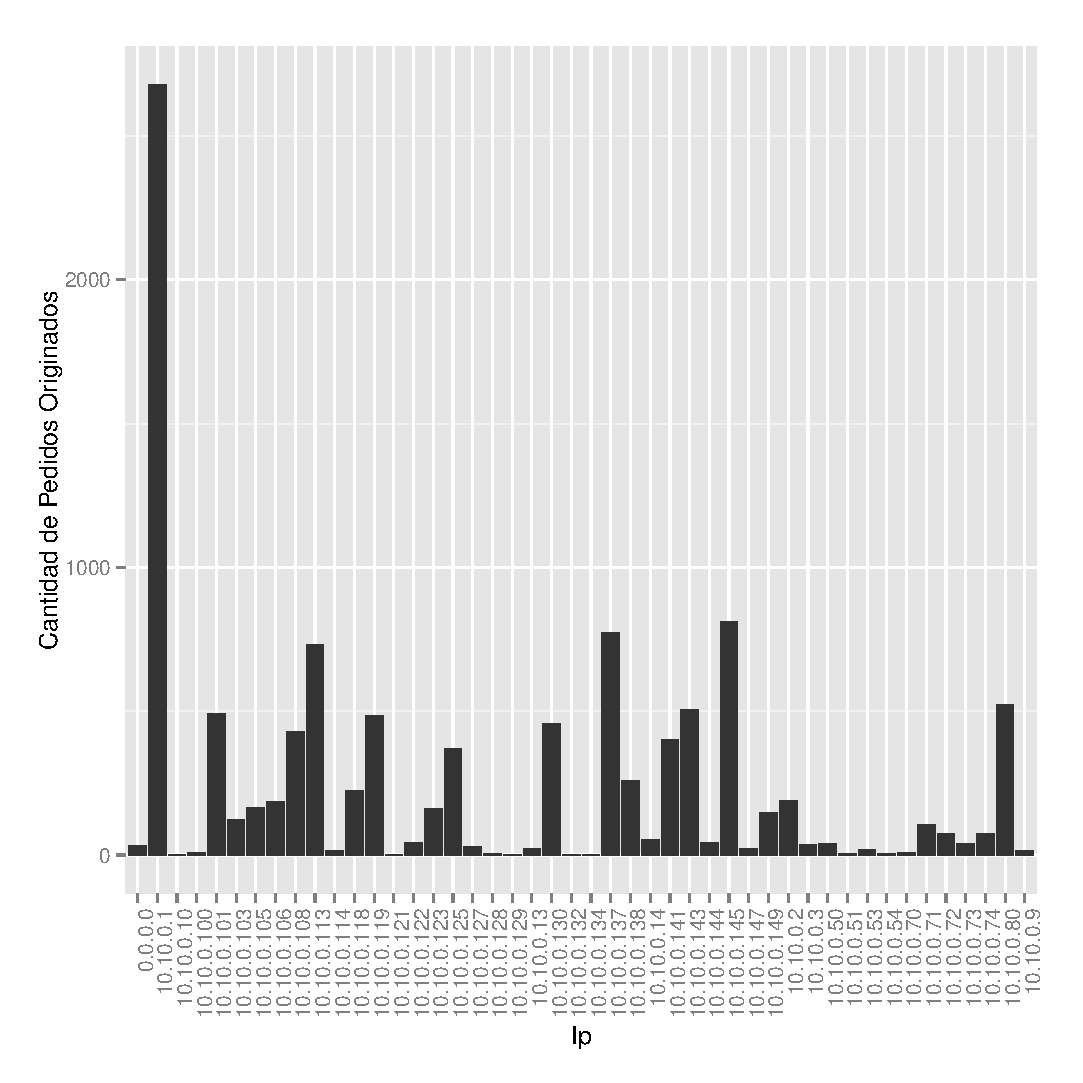
\includegraphics[width=0.5\textwidth]{img/graph/escenario_2/histogramSrc.eps}
		\caption{Escenario 2 - Histograma Origen}
		\label{fig:escenario2_histogramaSrc}
	\end{figure}       
    En este histograma podemos observar que hay una IP que predomina ampliamente sobre las demás, la 10.10.0.1, casualmente la del gateway. El resto se encuentra bastante distribuido. Hay 25 IPs que realizaron menos de 100 pedidos, 15 que realizaron entre 100 y 500, 5 que realizaron entre 500 y 1000 y el caso excepcional de la 10.10.0.1 que realizo 2678. Rapidamente nos dimos cuenta de no ibamos a obtener demasiada información sobre la red mirando quien origina los pedidos, porque lo importante es cuales son más solicitadas.
       
    \begin{figure}[!h]
		\centering
		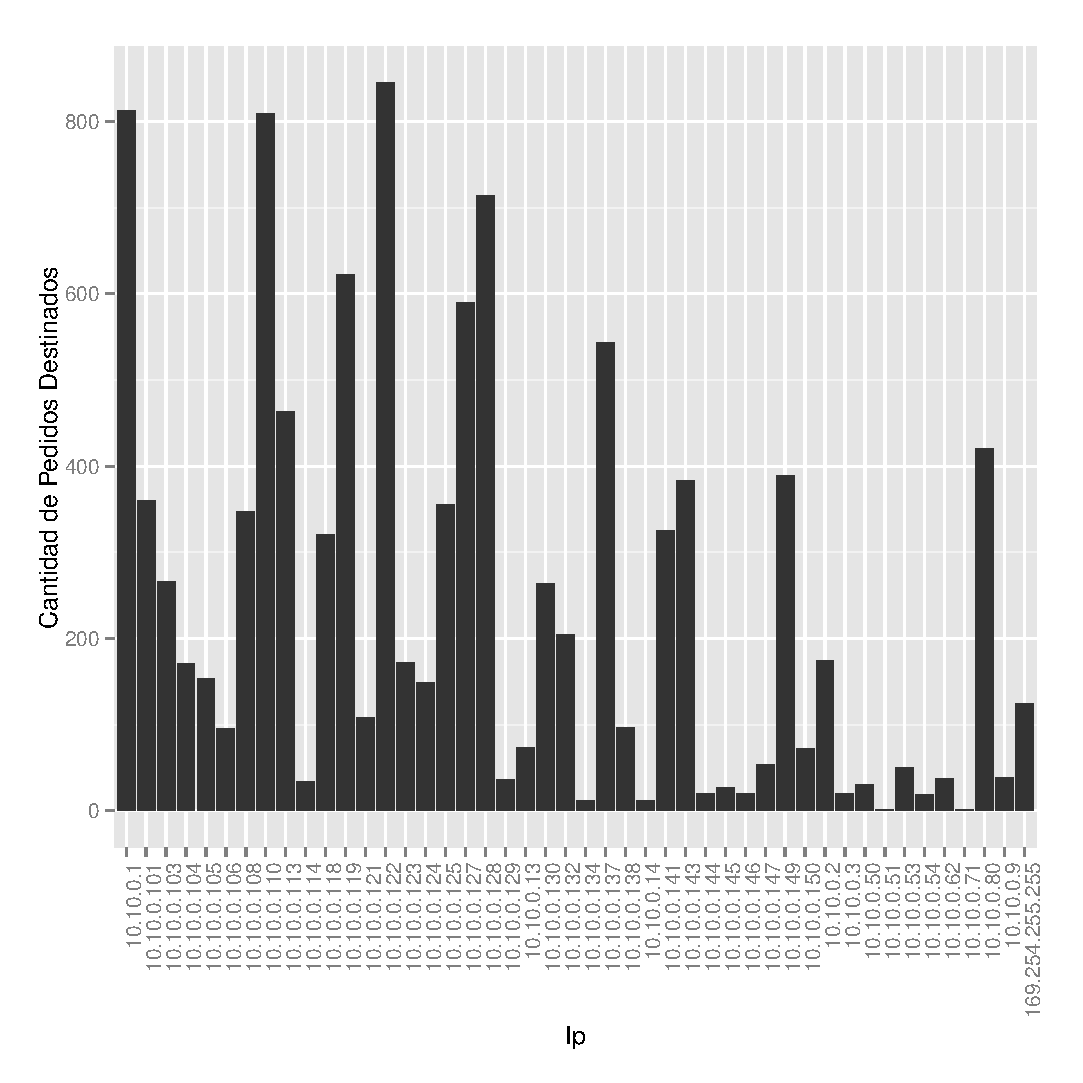
\includegraphics[width=0.5\textwidth]{img/graph/escenario_2/histogramDst.eps}
		\caption{Escenario 2 - Histograma Destino}
		\label{fig:escenario2_histogramaDst}
	\end{figure}
            
    \par En este otro histograma se ve una mayor distribución de los pedidos. Hay algunas IP que casí no cuentan con pedidos, mientras que hay muchas que cuentan con más de 100. Concretamente hay 20 IPs que fueron pedidas menos de 100 veces, 19 entre 100 y 500 veces y 7 pedidas entre 500 y 845 veces.
    Decidimos tomar las 5 IPs que fueron pedidas mayor cantidad de veces, para ver si nos aportaban alguna información valiosa:
        
    \begin{table}[!ht]
		\caption{Escenario 2 - IPs más pedidas}
		\centering
		\begin{tabular}{c c}
          IP & Cantidad de pedidos \\
          \hline 
          10.10.0.122 & 845 \\ 
          10.10.0.1 & 813 \\
          10.10.0.110 & 809 \\
          10.10.0.128 & 714 \\
          10.10.0.119 & 622 \\   
  		\end{tabular}
  	\end{table}
    
    En base a esto, buscamos en el grafo las vecindades de los nodos correspondientes a estas IPs:
    \begin{figure}[!ht]
		\centering
		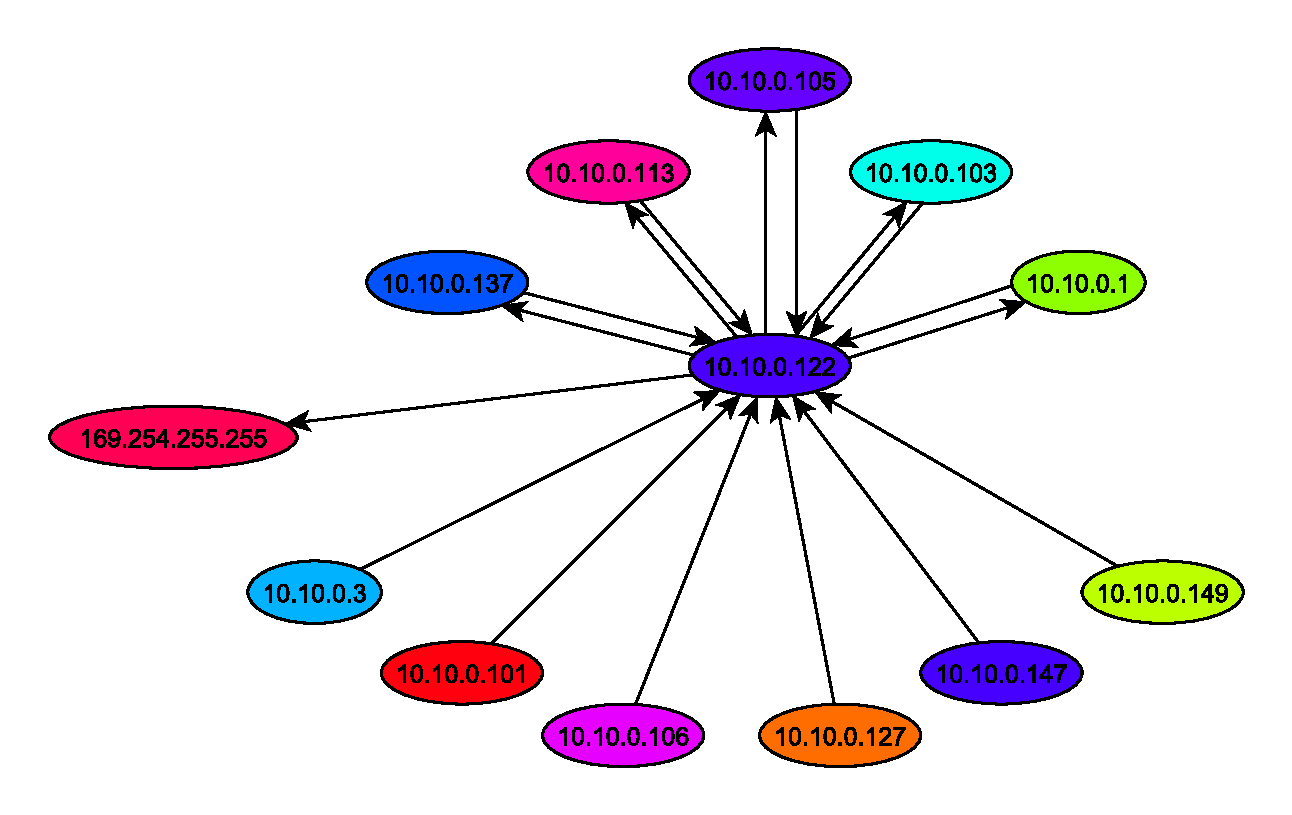
\includegraphics[width=0.5\textwidth]{img/graph/escenario_2/vecindad122.eps}
		\caption{Escenario 2 - Vecindad 10.10.0.122}
		\label{fig:escenario2_vecindad122}
	\end{figure}
    \begin{figure}[!ht]
		\centering
		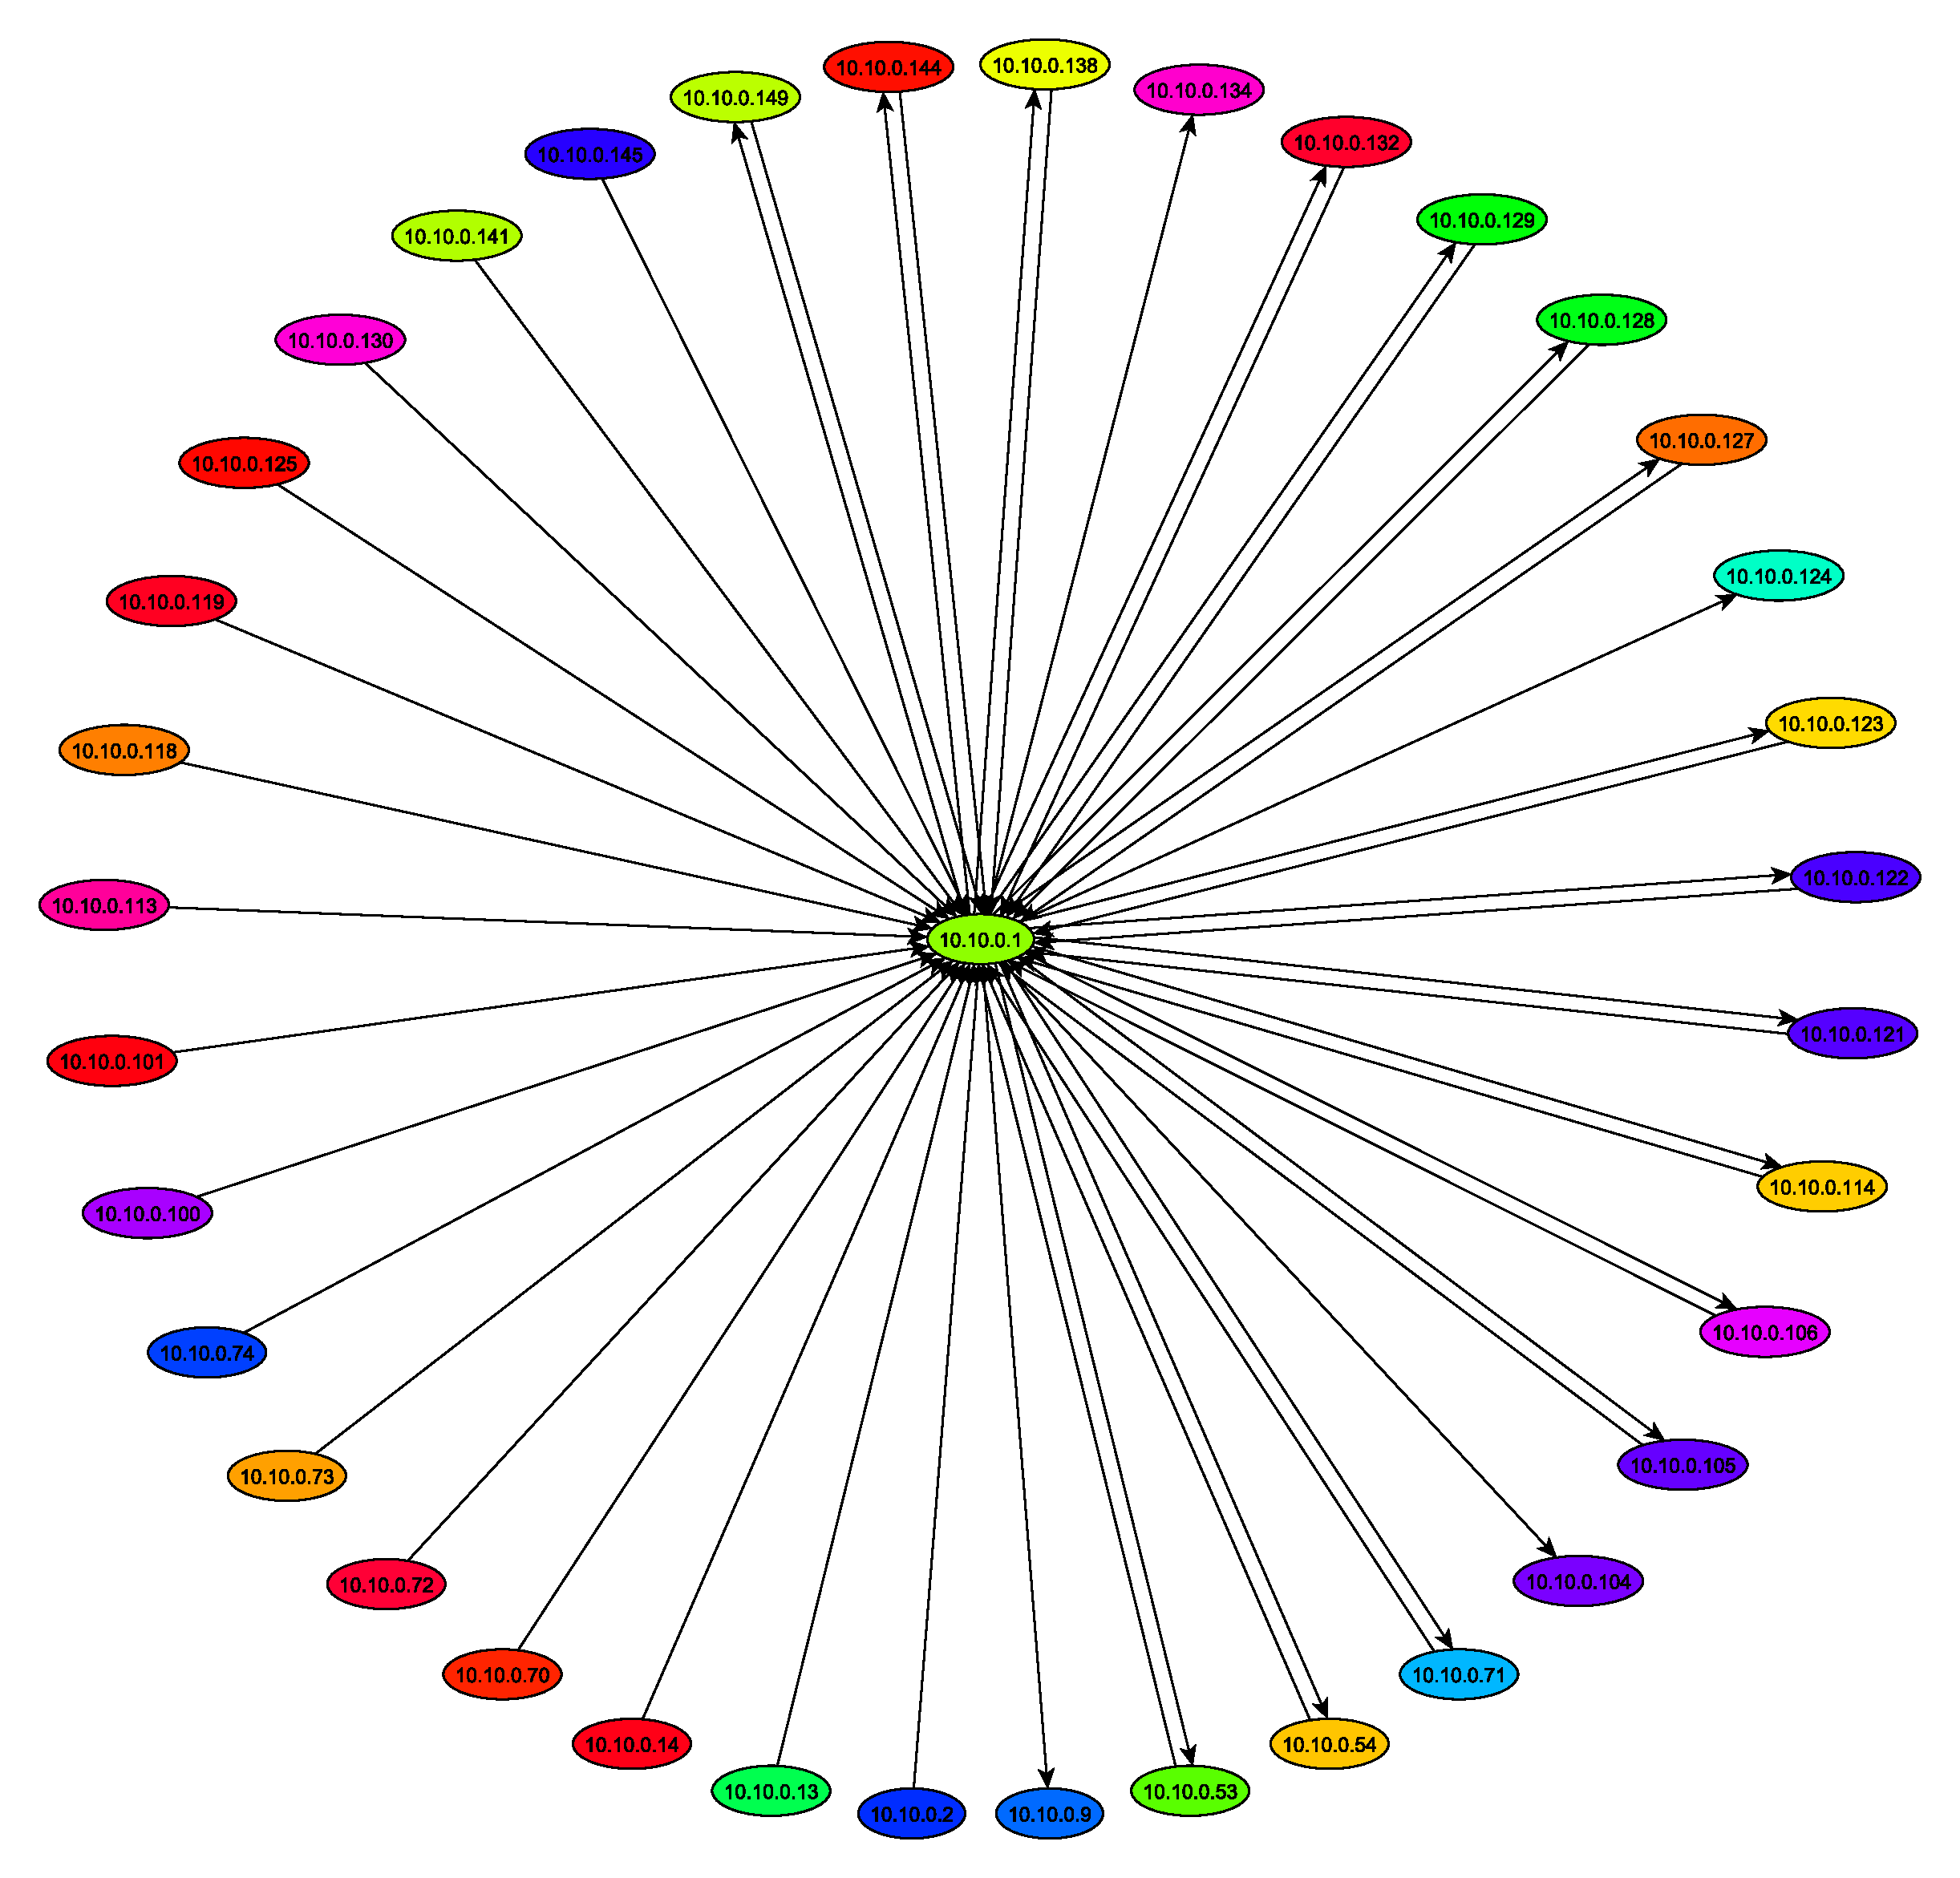
\includegraphics[width=0.5\textwidth]{img/graph/escenario_2/vecindad1.eps}
		\caption{Escenario 2 - Vecindad 10.10.0.1}
		\label{fig:escenario2_vecindad1}
	\end{figure}
    \begin{figure}[!ht]
		\centering
		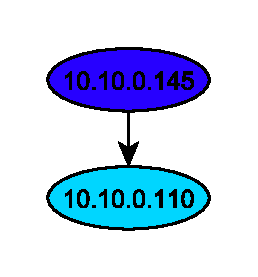
\includegraphics[width=0.25\textwidth]{img/graph/escenario_2/vecindad110.eps}
		\caption{Escenario 2 - Vecindad 10.10.0.110}
		\label{fig:escenario2_vecindad110}
	\end{figure}
    \begin{figure}[!ht]
		\centering
		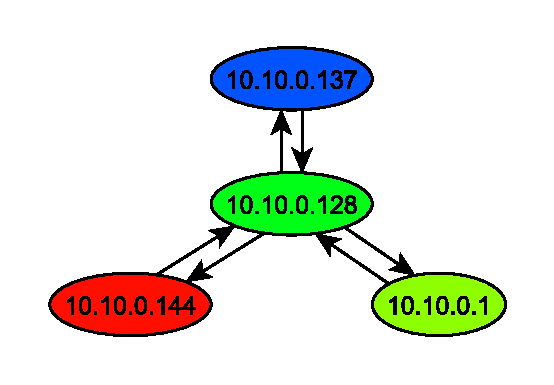
\includegraphics[width=0.5\textwidth]{img/graph/escenario_2/vecindad128.eps}
		\caption{Escenario 2 - Vecindad 10.10.0.128}
		\label{fig:escenario2_vecindad128}
	\end{figure}
    \begin{figure}[!ht]
		\centering
		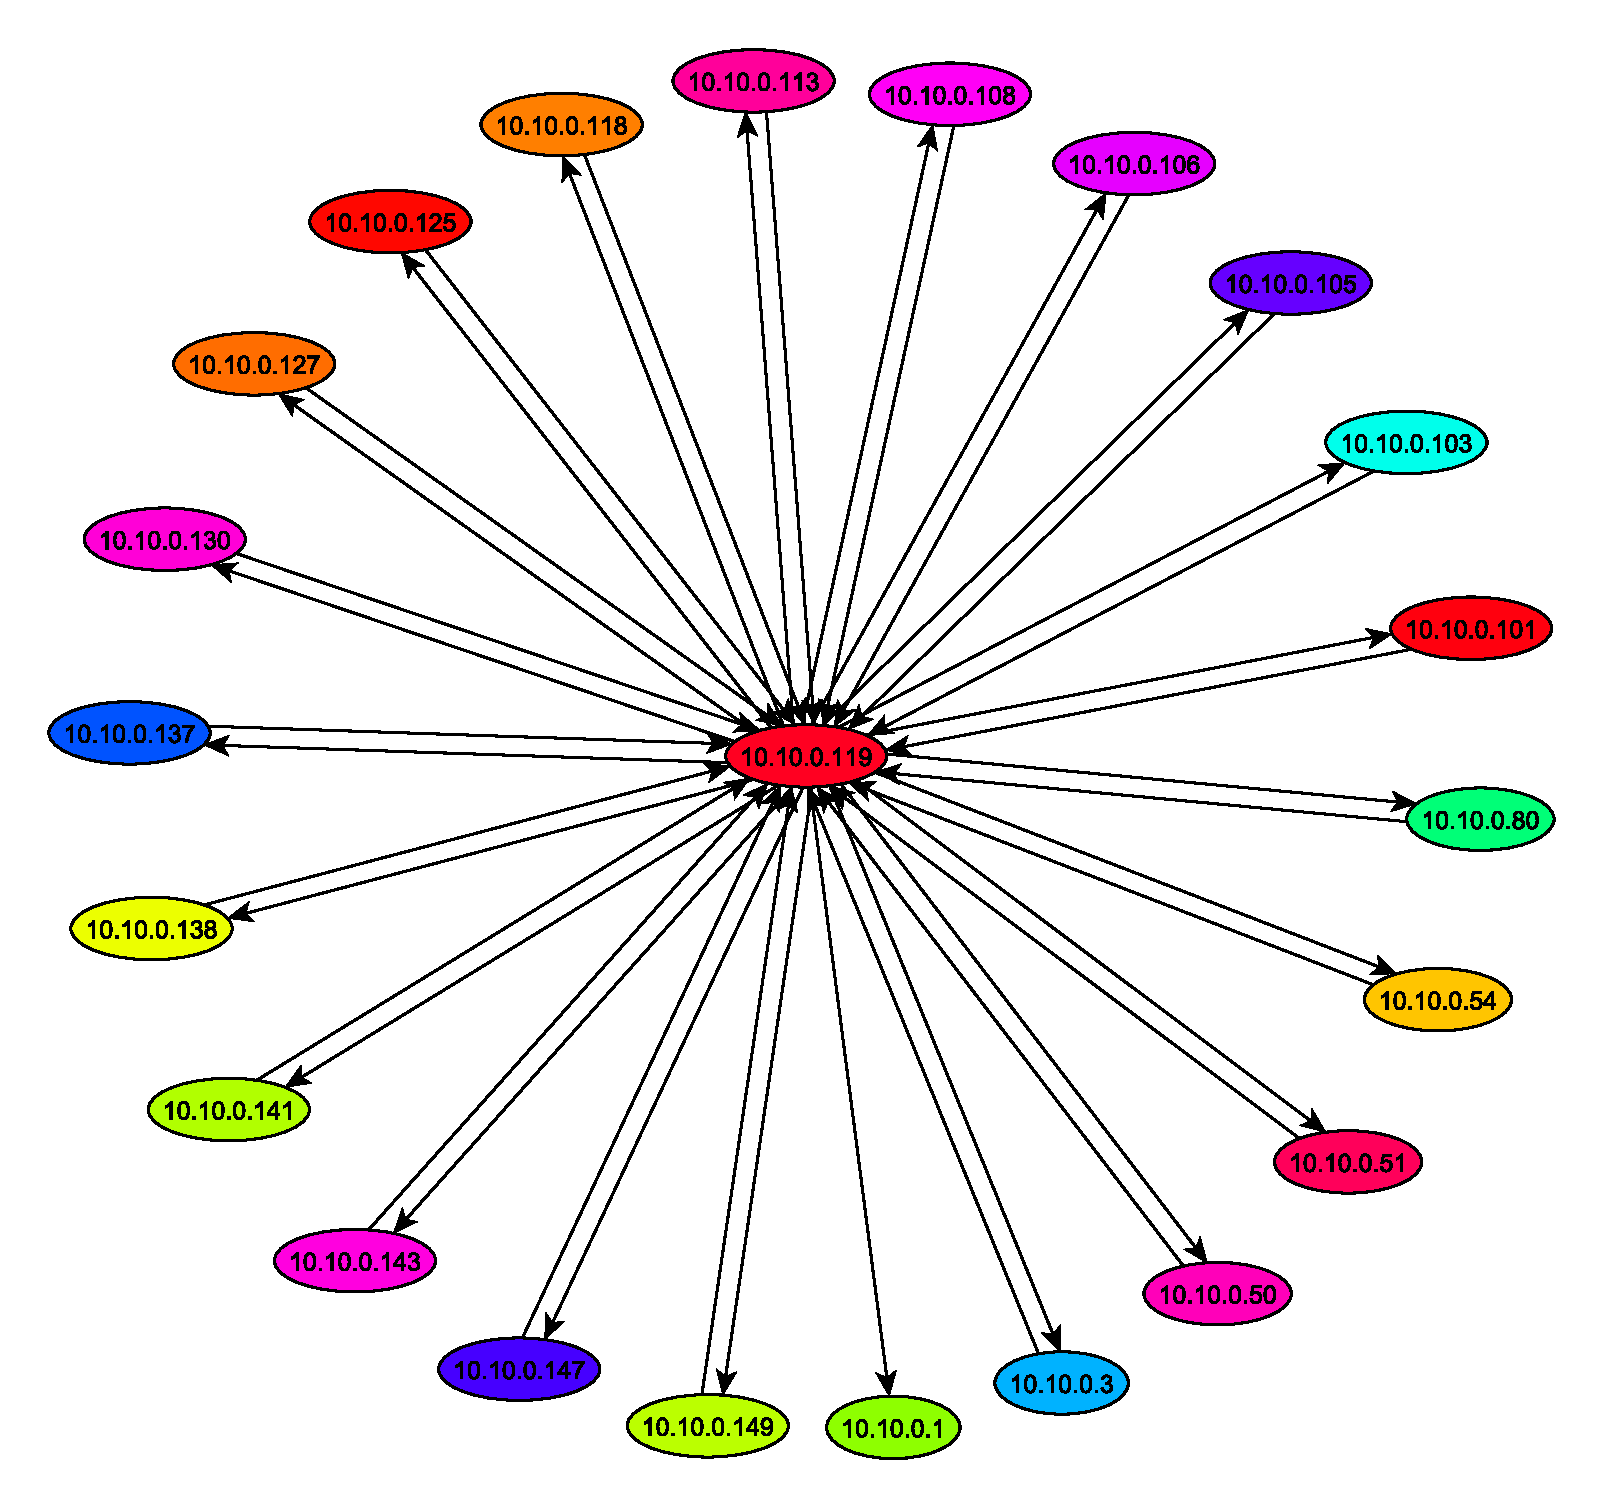
\includegraphics[width=0.5\textwidth]{img/graph/escenario_2/vecindad119.eps}
		\caption{Escenario 2 - Vecindad 10.10.0.119}
		\label{fig:escenario2_vecindad119}
	\end{figure}
    Acá notamos que 3 de las IPs tienen vecindades pobladas, lo que significa que seguramente sean nodos importantes en la red, mientras que en las otras dos se encuentran casí vacías.
    \par En el caso de la IP 10.10.0.110 vemos que esta no envió ningun pedido, por lo que es probable que no exista un host con esa IP, y que el equipo con IP 10.10.0.145 tuvierá configurado algún servicio que le pegue a la misma, y al no obtener respuesta, siguiera intentando continuamente, llenando de pedidos la red. Para corroborar una parte de esto, realizamos un ping hacia la IP 10.10.0.110 y vimos que efectivamente no existía.
    \par La IP 10.10.0.128 sabemos que existe en la red, ya que se ve que envía pedidos a otras IP, por lo que inspeccionamos con mayor detalle los pedidos dirigidas a esta. Nos llamo la atención que de los 714, 579 provenian del gateway. Aún más, los 579 se originaron en un rango 16 minutos, en los que la IP 10.10.0.128 no emitió ningún pedido. La conclusión que sacamos de esto es que probablemente esa dirección estuviera asignada a un teléfono celular, y que el dueño del mismo salió durante esos 15 minutos, por lo que el gateway comenzó a reintentar los pedidos al ver que no obtenía respuesta para esa IP.
    \par Nos resta inspeccionar las IPs 10.10.0.119 y 10.10.0.122 (la 10.10.0.1 ya sabemos que es el gateway, por lo que tiene sentido que tenga muchos pedidos, y en el grafo de su vecindad se puede apreciar la variedad de equipos qe la solicitan). 
    \par Por lo que aprendimos de los casos anteriores, nuestro primer intento para ver si realmente son nodos importantes, o son solo anomalías, va a ser graficar la cantidad de pedidos a estas IPs en franjas de media hora. De esta manera, si vemos una gran concentración de pedidos en poco tiempo, sabremos que nos encontramos con un caso similar al anterior, caso contrario, tenemos un potencial nodo importante.
    \begin{figure}[H]
		\centering
		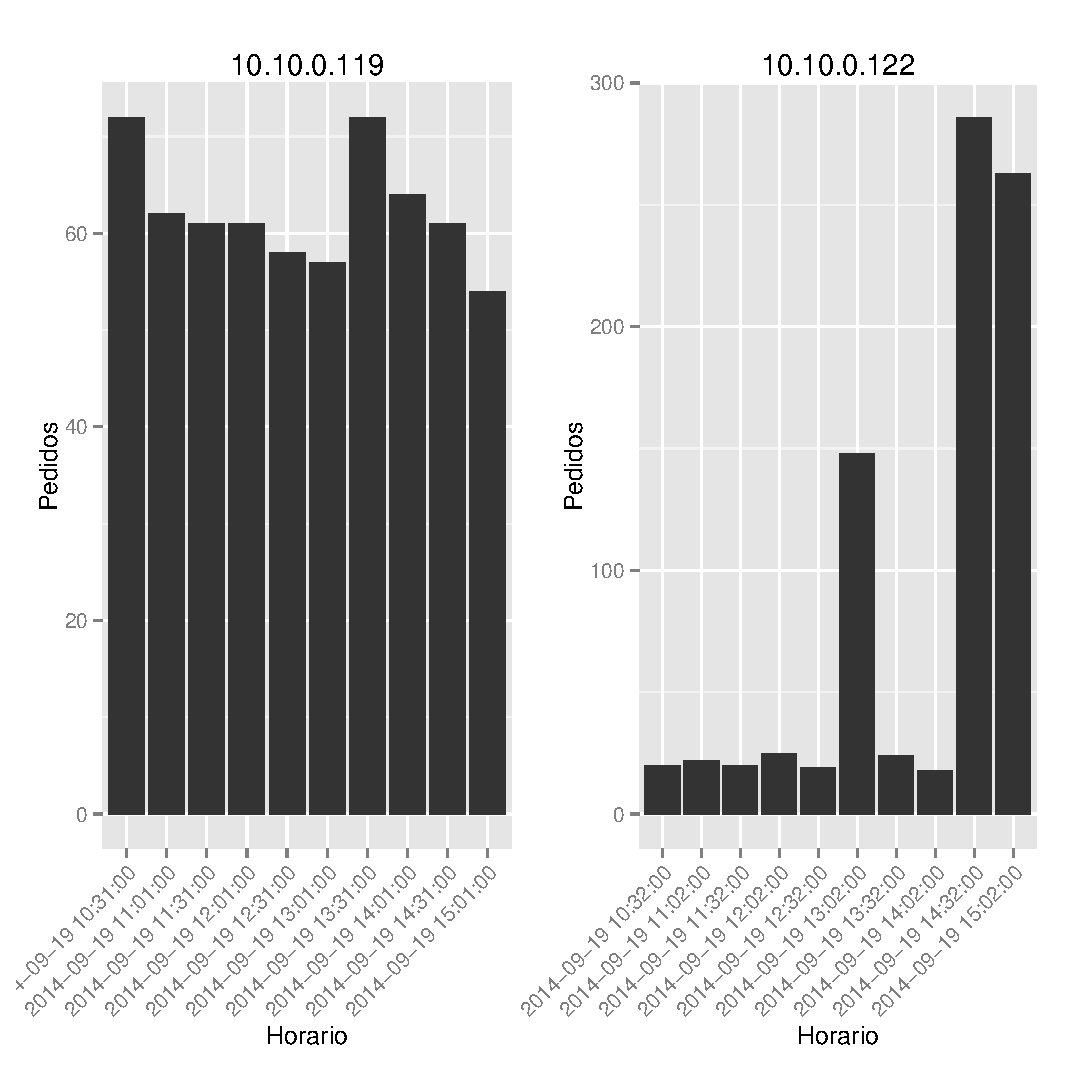
\includegraphics[width=0.5\textwidth]{img/graph/escenario_2/requestsCadaMediaHora119y122.eps}
		\caption{Escenario 2 - Pedidos cada media hora}
		\label{fig:escenario2_requestsCadaMediaHora119y122}
	\end{figure}
    \par Para el caso de la IP 10.10.0.119 vemos que hay una distribución pareja de los pedidos a lo largo del tiempo, por lo que podemos concluir en que es un nodo importante. 
    \par Por otro lado, en la IP 10.10.0.122 vemos que hay dos picos de pedidos en determinados horarios, y en el resto del tiempo de captura una cantidad muy baja (menos de 30 en cada franja), por lo que nos encontramos en una situación muy parecida a la de la IP 10.10.0.128. Preguntando quien tenía una máquina con esta IP, nos encontramos con que era una notebook, por lo que tiene sentido que el equipo se haya ido de la red (por ejemplo si el dueño se fue de la oficina y se la llevó con el).
    \par Por lo tanto, hasta el momento encontramos una única IP, aparte del gateway, que parece ser importante. Como esto no nos conforma, decidimos encarar de otra manera la búsqueda: En lugar de buscar por cantidad de pedidos que se le hiceron (cosa que ya vimos que no es demasiado util), vamos a buscar los nodos que más IPs distintas pidieron por ella, es decir, los nodos del grafo que tengan mayor grado de entrada.    
    \begin{table}[H]
		\caption{Escenario 2 - IPs con mayor grado de entrada}
		\centering
		\begin{tabular}{c c}
          IP & Cantidad de IPs distintas que la solicitaron \\
          \hline 
          10.10.0.1 & 32 \\ 
          10.10.0.113 & 21 \\
          10.10.0.119 & 21 \\
          10.10.0.80 & 19 \\
          10.10.0.137 & 19 \\   
  		\end{tabular}
  	\end{table}
    \par En este análisis si aparece como ganadora indiscutida la IP del gateway. Para corroborar que no nos encontramos con el mismo problema de los equipos que se van de la red y pasan a ser floodeados de pedidos de muchas IPs, graficamos la distribución de pedidos a cada una de ellas:
    \begin{figure}[H]
		\centering
		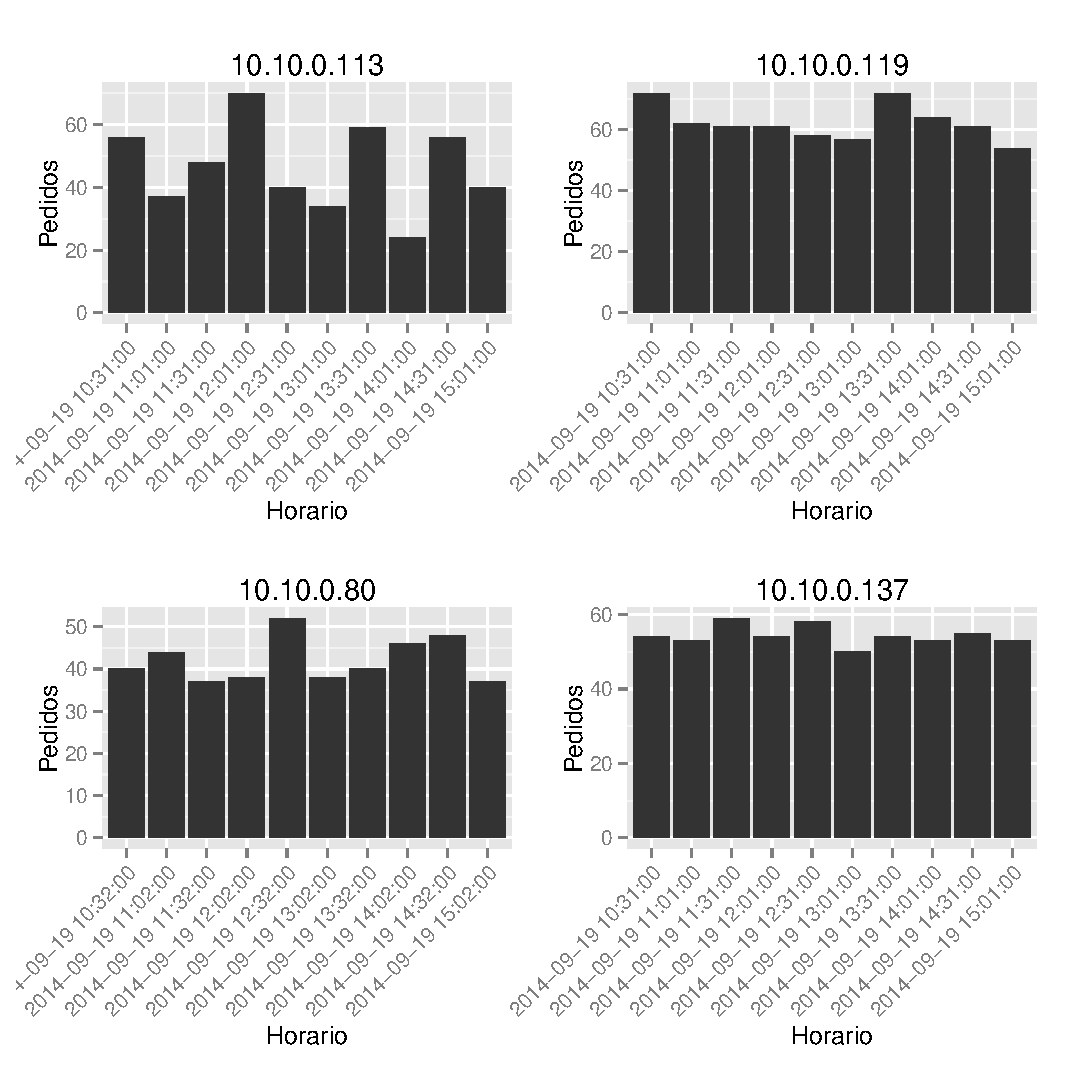
\includegraphics[width=0.5\textwidth]{img/graph/escenario_2/distribucionHoraria4IPsMasPedidas.eps}
		\caption{Escenario 2 - Pedidos cada media hora}
		\label{fig:escenario2_distribucionHoraria4IPsMasPedidas}
	\end{figure}
    \par Efectivamente, en todas las IP se ve en mayor o menor medida una distribución pareja de los pedidos a lo largo del día. En base a este analisis entonces también podemos concluir que estas IP son significativas en la red.
        
	\par Entrop\'ia

\subsection{Conclusiones Preliminares}